\definecolor{bostonuniversityred}{rgb}{0.8, 0.0, 0.0}
\newcommand{\aspas}[1]{``#1''}

\section{Melhoria de performance}

\subsection{Inversão de Loops}

\begin{frame}[fragile]{Inversão de \textit{loops}}
	\begin{columns}
		\column{0.4\linewidth}
			Consideremos o código.
		\column{0.6\linewidth}
			\begin{minted}[mathescape, linenos, numbersep=3pt, gobble=2, tabsize=4, frame=lines, framesep=2mm, fontsize=\footnotesize]{c++}
				for {i = l; i < n; i++)
					for (j =O; j <n; j++)
						a[i] [j] = 2 * a[i-1] [j];
			\end{minted}
	\end{columns}
	\begin{columns}
		\column{0.5\linewidth}
			\begin{itemize}
				\item Existe uma dependência de dados entre as linhas (\textbf{não podem ser executadas em paralelo}), mas não entre as colunas (\textbf{podem ser executadas em paralelo}).
			\end{itemize}
		\column{0.5\linewidth}
			\begin{figure}[H]
				\centering
				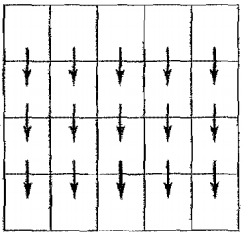
\includegraphics[width=0.3\linewidth]{img/quinn/diag-data-dep}
				\caption[Diagrama de dependência de dados]{Diagrama de dependência de dados}
				\label{fig:diag-data-dep}
			\end{figure}
	\end{columns}
\end{frame}

\begin{frame}[fragile]{Inversão de \textit{loops}}
	\begin{columns}
		\column{0.5\linewidth}
			\begin{itemize}
				\item Pode-se inverter o \textit{loop}, mantendo a coluna e alterando a linha.
				\medskip
				\item Dessa maneira, diferentes colunas podem ser executadas simultaneamente.
			\end{itemize}
		\column{0.5\linewidth}
			\begin{minted}[mathescape, linenos, numbersep=3pt, gobble=2, tabsize=4, frame=lines, framesep=2mm, fontsize=\footnotesize]{c++}
				#pragma omp parallel for private(i)
				for {i = l; i < n; i++)
					for (j =O; j <n; j++)
						a[i] [j] = 2 * a[i-1] [j];
			\end{minted}
	\end{columns}
\end{frame}

\subsection{Executando Loops Condicionais}

\begin{frame}[fragile]{\textit{Loops} Condicionais}
	\begin{itemize}
		\item Nem sempre é vantagem é vantajoso paralelizar código de um \textit{loop} entre múltiplas \textit{threads}:
		\medskip
		\begin{itemize}
			\item O \textit{loop} pode ter poucas iterações.
			\smallskip
			\item Dessa maneira, o \textit{overhead} de \textit{fork} e \textit{join} desvaloriza o \textit{speedup} do paralelismo.
		\end{itemize}
		\medskip
		\item Um exemplo pode ser o seguinte código, que calcula $\pi$ usando a regra do retângulo.
	\end{itemize}
	\begin{columns}
		\column{0.5\linewidth}
		\begin{minted}[mathescape, linenos, numbersep=3pt, gobble=2, tabsize=4, frame=lines, framesep=2mm, fontsize=\footnotesize]{c++}
		area = 0.0;
		#pragma omp parallel for private(x) reduction(+:area)
		for(i=0; i < n; i++)
		{
			x = (i + 0.5)/n;
			area += 4.0/(1.0 + x * x);
		}
		pi = area/n;
		\end{minted}
		\column{0.5\linewidth}
		\begin{figure}[H]
			\centering
			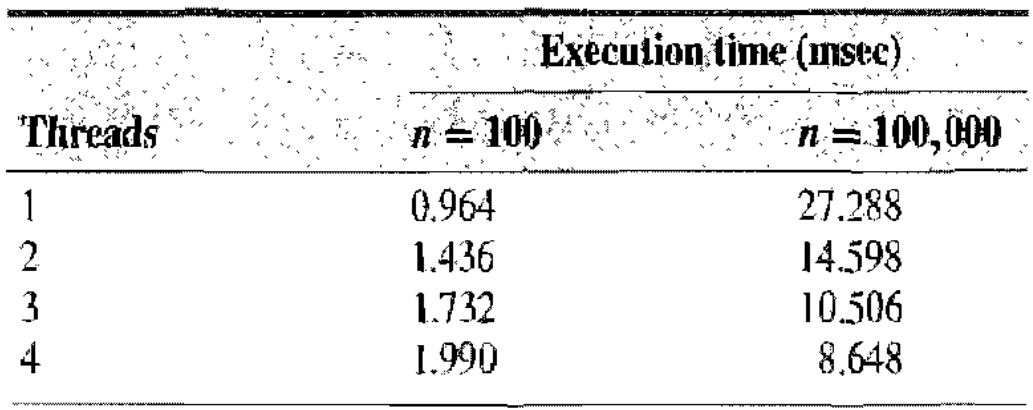
\includegraphics[width=0.8\linewidth]{img/quinn/tab-cond-loop}
			\caption[Comparação de performance entre múltiplas threads]{Comparação de performance entre múltiplas threads}
			\label{fig:tab-cond-loop}
		\end{figure}
	\end{columns}
	
\end{frame}

\begin{frame}[fragile]{\textit{Loops} Condicionais}
	\begin{itemize}
		\item A diretiva \texttt{if (<expressão>)} permite que sejam definidos os casos onde o \textit{loop} será executado paralelamente ou serialmente.
	\end{itemize}
		\begin{minted}[mathescape, linenos, numbersep=3pt, gobble=2, tabsize=4, frame=lines, framesep=2mm, fontsize=\footnotesize]{c++}
		area = 0.0;
		#pragma omp parallel for private(x) reduction(+:area) if(n > 500)
		for(i=0; i < n; i++)
		{
			x = (i + 0.5)/n;
			area += 4.0/(1.0 + x * x);
		}
		pi = area/n;
		\end{minted}
\end{frame}

\section{Diretivas, Cláusulas e Funções}

\begin{frame}{Diretivas, Cláusulas e Funções}
	\begin{itemize}
		\item Novas diretivas e cláusulas que serão vistas:
		\medskip
		\begin{itemize}
			\item \texttt{firstprivate} e \texttt{lastprivate}
			\medskip
			\item \texttt{sections}
			\medskip
			\item \texttt{parallel sections}
			\medskip
			\item \texttt{single}
			\medskip
			\item \texttt{nowait}
			\medskip
			\item \texttt{for}
		\end{itemize}
		\medskip
		\item Novas funções que serão vistas:
		\medskip
		\begin{itemize}
			\item \texttt{omp\_get\_num\_procs}
			\medskip
			\item \texttt{omp\_set\_num\_threads}
		\end{itemize}
	\end{itemize}
\end{frame}

\begin{frame}[fragile]{Funções}
	\begin{itemize}
		\item \texttt{omp\_get\_num\_procs}
		\medskip
		\begin{itemize}
			\item Retorna a quantidade de processadores disponíveis na máquina para execução do programa em paralelo.
			\smallskip
			\item Pode ser menor que a quantidade real, dependendo de como o sistema fornece acesso aos processadores pelos processos.
		\end{itemize}
		\medskip
		\item \texttt{omp\_set\_num\_threads}
		\begin{itemize}
			\item Define número de \textit{threads} para serem executadas em paralelo em uma seção de código.
			\smallskip
			\item Uso: \texttt{omp\_set\_num\_threads (int num\_threads)}.
			\smallskip
			\item Pode ser invocada múltiplas vezes ao longo do programa.
		\end{itemize}
		\medskip
		\item Um possível uso das duas funções juntas:
	\end{itemize}
	\begin{minted}[mathescape, linenos, numbersep=3pt, gobble=2, tabsize=4, frame=lines, framesep=2mm, fontsize=\footnotesize]{c++}
		int t;
		...
		t = omp_get_num_procs();
		omp_set_num_threads(t);
	\end{minted}
\end{frame}

\begin{frame}[fragile]{Cláusulas - firstprivate}
	\begin{columns}
		\column{0.3\linewidth}
		\begin{itemize}
			\item Suponhamos que temos esse código e desejamos paralelizá-lo.
		\end{itemize}
		\column{0.7\linewidth}
		\begin{minted}[mathescape, linenos, numbersep=3pt, gobble=2, tabsize=4, frame=lines, framesep=2mm, fontsize=\footnotesize]{c++}
			x[0] = complex_function();
			for (i=0; i < n; i++)
			{
				for(j=1; j < 4; j++)
					x[j] = g(i, x[j-1]);
				answer[i] = x[1] - x[3];
			}
		\end{minted}
	\end{columns}
	\pause
	\begin{itemize}
		\item Duas ressalvas:
		\smallskip
		\begin{enumerate}
			\item a função \texttt{g()} não tem efeitos colaterais.
			\smallskip
			\item Para evitar o \textit{overhead} de \textit{fork} e \textit{join} vamos paralelizar somente o \textit{loop} externo.
		\end{enumerate}
		\pause
		\item Para paralelizar o código, precisamos deixar as variáveis \textbf{j} e \textbf{x} privadas. ({\color{bostonuniversityred}Por que?})
		\pause
		\smallskip
		\item Podemos usar a diretiva \texttt{private}, porém, os valores de \textbf{x} serão inicializados com o valor padrão e não com o valor retornado pela função \texttt{complex\_function()}.
	\end{itemize}
\end{frame}

\begin{frame}[fragile]{Cláusulas - firstprivate}
	\begin{itemize}
		\item Usa-se então a diretiva \texttt{firstprivate}:
		\medskip
		\begin{itemize}
			\item Utiliza o valor armazenado atualmente na variável \textbf{compartilhada} para atribuir para cada uma das variáveis \textbf{privadas} criadas para cada \textit{thread}.
		\end{itemize}
	\end{itemize}
	\begin{minted}[mathescape, linenos, numbersep=3pt, gobble=2, tabsize=4, frame=lines, framesep=2mm, fontsize=\footnotesize]{c++}
		x[0] = complex_function();
		#pragma omp parallel for private(j) firstprivate(x)
		for (i=0; i < n; i++)
		{
			for(j=1; j < 4; j++)
				x[j] = g(i, x[j-1]);
			answer[i] = x[1] - x[3];
		}
	\end{minted}
\end{frame}

\begin{frame}[fragile]{Cláusulas - lastprivate}
	\begin{itemize}
		\item Podemos querer retornar um valor calculado na última iteração de um \textit{loop}, armazenado em uma variável privada, para a \textit{thread} mestre.
	\end{itemize}
	\begin{columns}
		\column{0.3\linewidth}
			\begin{itemize}
				\item Suponhamos o código já paralelizado.
			\end{itemize}
		\column{0.7\linewidth}
		\begin{minted}[mathescape, linenos, numbersep=3pt, gobble=2, tabsize=4, frame=lines, framesep=2mm, fontsize=\footnotesize]{c++}
		#pragma omp parallel for private(j)
		for (i=0; i < n; i++)
		{
			x[0] = 1.0;
			for (j=1; j < 4; j++)
				x[j] = x[j-1] * (i+1);
			sum_of_powers[i] = x[0] + x[1] + x[2] + x[3];
		}
		n_cubed = x[3];
		\end{minted}
	\end{columns}
	\begin{itemize}
		\item \texttt{x[3]} tem o valor de $n^3$, é interessante ter esse valor acessível fora do \texttt{parallel for}.
	\end{itemize}
\end{frame}

\begin{frame}[fragile]{Cláusulas - lastprivate}
	\begin{itemize}
		\item Usando a diretiva \texttt{lastprivate}:
	\end{itemize}
	\begin{minted}[mathescape, linenos, numbersep=3pt, gobble=2, tabsize=4, frame=lines, framesep=2mm, fontsize=\footnotesize]{c++}
		#pragma omp parallel for private(j) lastprivate(x)
		for (i=0; i < n; i++)
		{
			x[0] = 1.0;
			for (j=1; j < 4; j++)
				x[j] = x[j-1] * (i+1);
			sum_of_powers[i] = x[0] + x[1] + x[2] + x[3];
		}
		n_cubed = x[3];
	\end{minted}
	\begin{itemize}
		\item As diretivas \texttt{firstprivate} e \texttt{lastprivate} podem ser usadas simultaneamente, utilizando as mesmas variáveis entre si.
	\end{itemize}
\end{frame}

\begin{frame}[fragile]{Diretivas - for}
	\begin{columns}
		\column{0.3\linewidth}
		\begin{itemize}
			\item Suponhamos o seguinte código que queremos paralelizar.
		\end{itemize}
		\column{0.7\linewidth}
		\begin{minted}[mathescape, linenos, numbersep=3pt, gobble=2, tabsize=4, frame=lines, framesep=2mm, fontsize=\footnotesize]{c++}
		for (i = 0; i < m; i++)
		{
			low = a[i];
			high = b[i];
			if (low > high)
			{
				printf("Exiting during the iteration %d\n", i);
				break;
			}
			for (j = low; j < high; j++)
				c[j] = (c[j] - a[i])/b[i];
		}
		\end{minted}
	\end{columns}
	\fontsize{8pt}{7.2}\selectfont
	\begin{itemize}
		\item \textbf{Questão:} Podemos paralelizar \textbf{as iterações} do \textit{loop} mais externo?
		\pause
		\medskip
		\item {\color{bostonuniversityred} Não, existe o comando \textbf{break} no código, o que não caracteriza um \textbf{bloco estruturado de código}.}
		\pause
		\item Pode-se usar a cláusula \texttt{parallel for} no \textit{loop} mais interno.
		\pause
		\medskip
		%\fontsize{7.5pt}{7.2}\selectfont
		\begin{itemize}
			\item Porém, tem-se um \textit{overhead} maior de instruções de \textit{fork} e \textit{join} a cada iteração do \textit{loop} externo.
		\end{itemize}
	\end{itemize}
\end{frame}

\begin{frame}[fragile]{Diretivas - for}
	\begin{columns}
		\column{0.4\linewidth}
		\begin{itemize}
			\item Podemos adicionar a cláusula \texttt{parallel} no \textit{loop} externo.
			\smallskip
			\begin{itemize}
				\item Cada \textit{thread} vai executar todo o bloco de código.
				\smallskip
				\item Queremos que as iterações do \textit{loop} mais interno sejam divididas entre as \textit{threads}.
				\smallskip
				\item Para isso, usamos a diretiva \texttt{for}, que especifica que as iterações devem ser divididas.
				\smallskip
				\item Diferente da \texttt{parallel for} pois não faz o \textit{fork} e \textit{join}, apenas divide o trabalho em um bloco com a diretiva \texttt{parallel}.
			\end{itemize}
		\end{itemize}
		\column{0.6\linewidth}
		\begin{minted}[mathescape, linenos, numbersep=3pt, gobble=2, tabsize=4, frame=lines, framesep=2mm, fontsize=\footnotesize]{c++}
		#pragma omp parallel private(i,j)
		for (i = 0; i < m; i++)
		{
			low = a[i];
			high = b[i];
			if (low > high)
			{
				printf("Exiting during the iteration %d\n", i);
				break;
			}
			#pragma omp for
			for (j = low; j < high; j++)
				c[j] = (c[j] - a[i])/b[i];
		}
		\end{minted}
	\end{columns}
\end{frame}

\begin{frame}[fragile]{Diretivas - single}
	\begin{columns}
		\column{0.4\linewidth}
		\begin{itemize}
			\item Ainda analisando o mesmo exemplo, seria interessante se a mensagem de erro fosse imprimida apenas uma vez.
			\smallskip
			\item Usa-se então a diretiva \texttt{single} que especifica que somente uma \textit{thread} deve executa o bloco de código conseguinte.
		\end{itemize}
		\column{0.6\linewidth}
		\begin{minted}[mathescape, linenos, numbersep=3pt, gobble=2, tabsize=4, frame=lines, framesep=2mm, fontsize=\footnotesize]{c++}
		#pragma omp parallel private(i,j)
		for (i = 0; i < m; i++)
		{
			low = a[i];
			high = b[i];
			if (low > high)
			{
				#pragma omp single
				printf("Exiting during the iteration %d\n", i);
				break;
			}
			#pragma omp for
			for (j = low; j < high; j++)
				c[j] = (c[j] - a[i])/b[i];
		}
		\end{minted}
	\end{columns}
\end{frame}

\begin{frame}{Cláusulas - nowait}
	\begin{itemize}
		\item A diretiva \texttt{parallel} faz com que o compilador imponha uma barreira de sincronização.
		\medskip
		\item Cada \textit{thread} que termina uma iteração do \textit{loop} externo, deve esperar o término das outras \textit{threads} para executar a próxima iteração.
		\smallskip
		\begin{itemize}
			\item A alteração simultânea das variáveis \texttt{low} e \texttt{high} pode influenciar na execução das iterações nas outras \textit{threads}.
		\end{itemize}
		\medskip
		\item Se fizermos as variáveis \texttt{low} e \texttt{high} privadas, essa barreira é desnecessária.
		\medskip
		\item Pode-se remover a barreira de sincronização explicitamente com a diretiva \texttt{nowait}.
	\end{itemize}
\end{frame}

\begin{frame}[fragile]{Cláusulas - nowait}
		\begin{minted}[mathescape, linenos, numbersep=3pt, gobble=2, tabsize=4, frame=lines, framesep=2mm, fontsize=\footnotesize]{c++}
		#pragma omp parallel private(i,j,low,high)
		for (i = 0; i < m; i++)
		{
			low = a[i];
			high = b[i];
			if (low > high)
			{
				#pragma omp single
				printf("Exiting during the iteration %d\n", i);
				break;
			}
			#pragma omp for nowait
			for (j = low; j < high; j++)
				c[j] = (c[j] - a[i])/b[i];
		}
		\end{minted}
\end{frame}

\subsection{Paralelismo Funcional}

\begin{frame}[fragile]{Paralelismo Funcional}
	\begin{itemize}
		\item Além do paralelismo de dados, também existe o paralelismo funcional.
		\medskip
		\item A OpenMP permite a atribuição de diferentes \textit{threads} para diferentes porções de código.
		\medskip
		\item Podemos ver no código, que considerando que todas as funções não tem efeitos colaterais, \texttt{aplha}, \texttt{beta} e \texttt{delta} podem ser executadas em paralelo.
	\end{itemize}
	\begin{minted}[mathescape, linenos, numbersep=3pt, gobble=2, tabsize=4, frame=lines, framesep=2mm, fontsize=\footnotesize]{c++}
		v = alpha();
		w = beta();
		x = gamma(v, w);
		y = delta();
		printf ("%6.2f\n", epsilon(x,y));
	\end{minted}
\end{frame}
	
\begin{frame}[fragile]{Diretivas - parallel sections}
	\begin{itemize}
		\item Precede blocos de código que são especificados para serem executados em paralelo.
		\medskip
		\item Tem como sintaxe:
		\medskip
	\end{itemize}
	\begin{minted}[mathescape, linenos, numbersep=3pt, gobble=2, tabsize=4, frame=lines, framesep=2mm, fontsize=\footnotesize]{c++}
		#pragma omp parallel sections
	\end{minted}
\end{frame}

\begin{frame}[fragile]{Diretivas - section}
	\begin{itemize}
		\item Faz parte do bloco delimitado pela diretiva \texttt{parallel sections} (geralmente por chaves \{\}) e precede algum bloco de código.
		\medskip
		\item Seguindo com o exemplo apresentado:
	\end{itemize}
	\begin{minted}[mathescape, linenos, numbersep=3pt, gobble=2, tabsize=4, frame=lines, framesep=2mm, fontsize=\footnotesize]{c++}
		#pragma omp parallel sections
		{
			#pragma omp section
			v = alpha();
			#pragma omp section
			w = beta();
			#pragma omp section
			y = delta();
		}
		x = gamma(v, w);
		printf ("%6.2f\n", epsilon(x,y));
	\end{minted}
\end{frame}

\begin{frame}{Explorando o paralelismo funcional}
	\begin{itemize}
		\item Com o exemplo apresentado, se executarmos as funções \texttt{aplha}, \texttt{beta} e \texttt{delta} em paralelo, não existirão mais oportunidades de paralelismo funcional.
		\pause
		\medskip
		\item Porém, se executarmos apenas \texttt{aplha} e \texttt{beta} em paralelo, depois de obtidos os resultados, pode-se executar \texttt{gamma} e \texttt{delta} também em paralelo.
		\medskip
		\item Podem ser extraídas então quatro seções, divididas em dois grupos de seções.
		\medskip
		\item Pode-se usar a diretiva \texttt{parallel} para encapsular as duas seções, reduzindo o \textit{overhead} de \textit{fork} e \textit{join}
	\end{itemize}
\end{frame}

\begin{frame}[fragile]{Explorando o paralelismo funcional}
	\begin{minted}[mathescape, linenos, numbersep=3pt, gobble=2, tabsize=4, frame=lines, framesep=2mm, fontsize=\footnotesize]{c++}
		#pragma omp parallel
		{
			#pragma omp sections
			{
				#pragma omp section
				v = alpha();
				#pragma omp section
				w = beta();
			}
			#pragma omp sections
			{
				#pragma omp section
				x = gamma(v, w);
				#pragma omp section
				y = delta();
			}
		}
		printf ("%6.2f\n", epsilon(x,y));
	\end{minted}
\end{frame}

\begin{frame}{Sumário - OpenMP}
	\begin{figure}
		\centering
		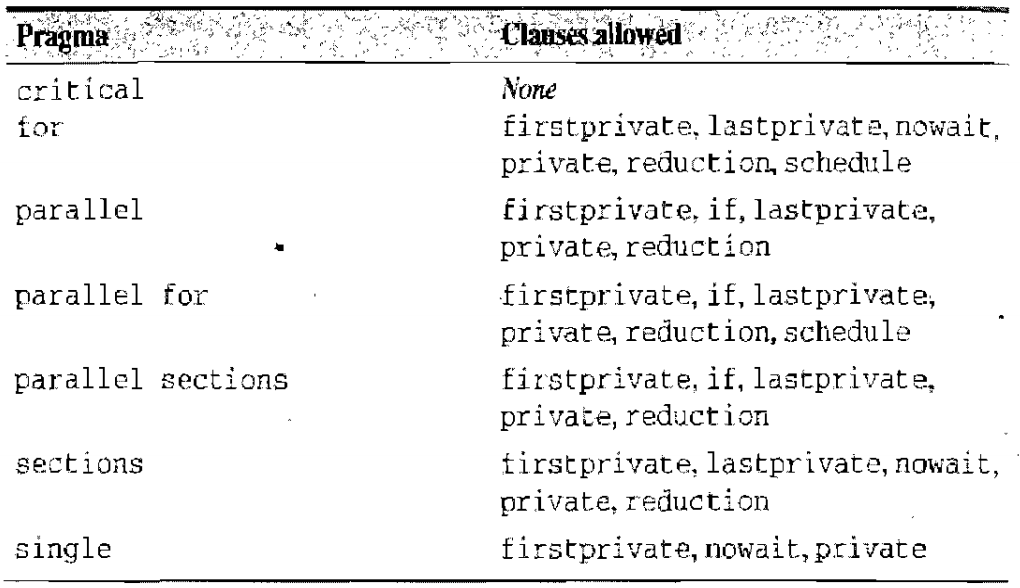
\includegraphics[width=0.8\linewidth]{img/quinn/sum-omp}
		\caption[Sumário de pragmas da OpenMP]{Sumário de pragmas da OpenMP}
		\label{fig:sum-omp}
	\end{figure}
\end{frame}

\section{Combinando OpenMP e MPI}

\begin{frame}{Combinando OpenMP e MPI}
	\begin{itemize}
		\item Atualmente temos acesso à multicomputadores, onde cada computador é um multiprocessador (\textbf{Ex:} \textit{Cluster}).
		\medskip
		\item Deseja-se, na execução de alguma aplicação, deixar todas os processadores de todos os computadores ativos e trabalhando.
		\medskip
		\item Podemos fazer isso com a MPI, criando processos $P_i$ para cada $n$ computador e cada $m$ processador (n $\times$ m processos).
		\medskip
		\item  Algum problema? \pause \textbf{{\color{bostonuniversityred} \textit{Overhead} desnecessário de comunicação através de troca de mensagens!}}
		\pause
		\medskip
		\item Pode-se, com a MPI, criar processos $P_i$ para cada $n$ computador e $k$ \textit{threads} $t_i$ para cada processador em cada computador, utilizando a OpenMP.
		\medskip
		\item \textit{Threads} precisam armazenar menos informações do que processos, sendo \aspas{mais leves}
	\end{itemize}
\end{frame}

\begin{frame}{Combinando OpenMP e MPI}
	\begin{figure}
		\centering
		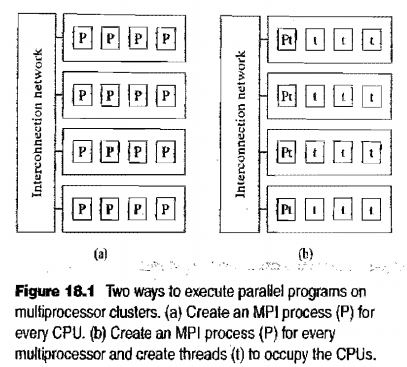
\includegraphics[width=0.6\linewidth]{img/quinn/openMP+MPI}
		\caption[Combinando OpenMP e MPI]{Combinando OpenMP e MPI}
		\label{fig:openMP+MPI}
\end{figure}
\end{frame}

%\begin{frame}{Exemplo - Método de Gradiente Conjugado}
%	\begin{itemize}
%		\item Nesse exemplo, um código totalmente em MPI será convertido em uma implementação híbrida de OpenMP + MPI.
%		\medskip
%		\item Método para resolução de um sistema linear de equações na forma $Ax = b$.
%		\medskip
%		\item Funções do método: 
%		\smallskip
%		\begin{itemize}
%			\item \texttt{main}: Método principal, com funções de início e término da MPI.
%			\smallskip
%			\item \texttt{cg}: Resolve de fato o sistema $Ax = b$ e imprime a solução.
%			\smallskip
%			\item \texttt{dot\_product}: Produto escalar de dois vetores, cada processo tem sua cópia do vetor.
%			\smallskip
%			\item \texttt{matrix\_vector\_product}: Produto de matriz por vetor. É feita uma divisão de linhas para os processos, com vetores replicados (\textbf{Será o foco desse exemplo}).
%		\end{itemize}
%	\end{itemize}
%\end{frame}

\begin{frame}[fragile]{Exemplo - Hello World}
	\begin{minted}[mathescape, linenos, numbersep=3pt, gobble=2, tabsize=4, frame=lines, framesep=2mm, fontsize=\fontsize{8.5}{7.2}\selectfont]{c++}
		#include <stdio.h>
		#include "mpi.h"
		#include <omp.h>
		
		int main(int argc, char *argv[]){
			int numprocs, rank, namelen;
			char processor_name[MPI_MAX_PROCESSOR_NAME];
			int t_id = 0, nt = 1;
			
			MPI_Init(&argc, &argv);
			MPI_Comm_size(MPI_COMM_WORLD, &numprocs);
			MPI_Comm_rank(MPI_COMM_WORLD, &rank);
			MPI_Get_processor_name(processor_name, &namelen);
			
			#pragma omp parallel default(shared) private(iam, np)
			{
				nt = omp_get_num_threads();
				t_id = omp_get_thread_num();
				printf("Hello from thread %d out of %d from process %d out of %d on %s\n",
					t_id, nt, rank, numprocs, processor_name);
			}
			
			MPI_Finalize();
		}
	\end{minted}
\end{frame}

\begin{frame}[fragile]{Exemplo - Compilando e Executando}
	\begin{itemize}
		\item Compilando:
	\end{itemize}
	\begin{minted}[mathescape, linenos, numbersep=3pt, gobble=2, tabsize=4, frame=lines, framesep=2mm, fontsize=\footnotesize]{bash}
		$ mpicc -openmp hello.c -o hello
	\end{minted}
	\begin{itemize}
		\item Executando:
	\end{itemize}
	\begin{minted}[mathescape, linenos, numbersep=3pt, gobble=2, tabsize=4, frame=lines, framesep=2mm, fontsize=\footnotesize]{bash}
		$ export OMP_NUM_THREADS=4
		$ mpirun -x OMP_NUM_THREADS ./hello
	\end{minted}
\end{frame}

\begin{frame}{Exemplo - Possível saída}
	\begin{alertblock}{Saída}
		Hello from thread 0 out of 4 from process 0 out of 2 on morab006\\
		Hello from thread 1 out of 4 from process 0 out of 2 on morab006\\
		Hello from thread 2 out of 4 from process 0 out of 2 on morab006\\
		Hello from thread 3 out of 4 from process 0 out of 2 on morab006\\
		Hello from thread 0 out of 4 from process 1 out of 2 on morab001\\
		Hello from thread 3 out of 4 from process 1 out of 2 on morab001\\
		Hello from thread 1 out of 4 from process 1 out of 2 on morab001\\
		Hello from thread 2 out of 4 from process 1 out of 2 on morab001
	\end{alertblock}
\end{frame}

\begin{frame}[fragile]{Mais Exemplos}
	\begin{itemize}
		\item Capítulo 18 do livro \textbf{Parallel Programming in C With Mpi and Openmp} do autor Michael J. Quinn:
		\medskip
		\begin{itemize}
			\item Método de Gradiente Conjugado.
			\medskip
			\item Método de Jacobi.
		\end{itemize}
	\end{itemize}
\end{frame}

\begin{frame}{Onde Adquirir OpenMP e MPI}
	\begin{itemize}
		\item OpenMP: Suporte do compilador.
		\medskip
		\begin{itemize}
			\item GCC (Gnu Compiler Collection): Versão $\geq$ 4.2 \footnote{\url{http://is.gd/MKkNVK}}, adiciona-se o parâmetro \texttt{-fopenmp}.
			\smallskip
			\item Clang: Versão $\geq$ 3.7 \footnote{\url{https://clang-omp.github.io/}}, adiciona-se o parâmetro \texttt{-fopenmp}.
		\end{itemize}
		\bigskip
		\item MPI é uma especificação, diferentes bibliotecas a implementam:
		\begin{itemize}
			\item MPICH: Dá suporte a C, Fortran e pouco suporte a C++. Disponível em \url{https://www.mpich.org/}.
			\smallskip
			\item Open MPI: Dá suporte a C, Fortran e C++. Disponível em \url{https://www.open-mpi.org/}.
			\smallskip
			\item Boost.MPI: Dá suporte a C++ e Python. Disponível em \url{http://www.boost.org/doc/libs/1_59_0/doc/html/mpi.html}.
		\end{itemize}
	\end{itemize}
\end{frame}

